% \begin{savequote}[8cm]
% Alles Gescheite ist schon gedacht worden.\\
% Man muss nur versuchen, es noch einmal zu denken.

% All intelligent thoughts have already been thought;\\
% what is necessary is only to try to think them again.
%   \qauthor{--- Johann Wolfgang von Goethe \cite{von_goethe_wilhelm_1829}}
% \end{savequote}

\chapter{\label{ch:genai}What Are Generative AI Detectors Good For? Evaluating and Implementing with the Decision Matrix}

\minitoc

\section{Introduction}\label{sec:intro}
Since \textcite{ashish_vaswani_attention_2017} introduced transformer architecture, AI has made rapid progress. More recently, large language models (LLMs) like BERT and GPT3 have demonstrated the ability to generate human-like text \cite{jacob_devlin_bert_2018,brown_language_2020}. The releases of GPT3.5 and GPT4o have made these models more powerful and ubiquitous, and students are increasingly using them to write essays \cite{openai_gpt-4_2023,dehouche_plagiarism_2021}. This has raised concerns about plagiarism, and while many generative AI (genAI)-users are caught by detectors, these detectors often fall short of their goal \cite{liang_gpt_2023,kalpesh_krishna_paraphrasing_2023,mitchell_detectgpt_2023,tharindu_kumarage_stylometric_2023,dehouche_plagiarism_2021}. Essay-writers' ability to use genAI has changed the role of essay-based teaching and evaluation, especially in competitive contexts like scholarship selection.

Many bodies of research seek to understand this new role. Among them, theoretical research attempts to determine what uses of genAI constitute plagiarism, or should otherwise be banned, and what uses do not \cite{yu_huang_reflection_2023,mike_perkins_decoding_2023}. Meanwhile, practical research builds and evaluates genAI detectors to determine whether a ban on such use is enforceable \cite{mitchell_detectgpt_2023,tharindu_kumarage_stylometric_2023,kalpesh_krishna_paraphrasing_2023}. However, theoretical accounts focus primarily on what constitutes plagiarism, and detectors and their evaluations are often concerned with detecting said plagiarism under adversarial assumptions \cite{yu_huang_reflection_2023,kalpesh_krishna_paraphrasing_2023}. Work that does not overtly concern itself with plagiarism still grapples with issues of detecting and removing cohorts or passages, inadvertently viewing the problem through a plagiarism lens \cite{mitchell_detectgpt_2023,liang_gpt_2023}. This focus on plagiarism neglects other problems genAI has created for practitioners.

We address this here with Action Research (AR). We partner and ``research with'' \cite{bradbury_action_2003} an anonymous scholarship and talent investment organisation to understand the needs of their team of scholarship selection practitioners (N=8; excludes authors) with regards to categorising and interpreting application essays and undertake this research while supporting their 2022 and 2023 application cycles. We identify ``decision points'' when the program requires or desires to make a decision we might support with contextual information about genAI usage (see Table \ref{tab:decisions}). Through conversations with internal stakeholders \cite{Hayes_2011}, we identify two axes, `stage' and `stakes', on which these decisions exist \cite{braun_using_2006}; we use these axes to construct the Decision Matrix in Figure \ref{fig:decision_matrix}. We then evaluate three genAI detectors on these decisions.

AR revealed a number of decisions that selection practitioners desire to make surrounding genAI. Though the literature focuses on the decision of whether or not to disqualify applicants using genAI, our partner organisation dismissed this decision as irrelevant, as their application guidelines do not forbid the usage of genAI. Instead, the program expressed interest in decisions such as diligence, where the program provides information about genAI usage alongside other facts about the applicant to make a holistic decision about when and how to consider an applicant. We conceptualise these decisions in a Decision Matrix with axes relating to their `stage' (i.e., where does this fit in the selection process?) and `stakes' (i.e., what is the magnitude of the consequence of this decision?). We then identify the properties desired from detectors in order that they might support different decisions on different parts of our Matrix. In our evaluation of detectors for these decisions, we find that organisational needs are not met by current detectors, particularly with regards to in-process decision-making. Our results suggest that detectors can be useful in aggregate analyses to support ex-post decisions. As a case study, we use one of our detectors, GPTZero, to support two decisions: \emph{Partners} and \emph{Pipeline} (described in Table \ref{tab:decisions}). We demonstrate two applications of detectors to the support of ex-post decisions. The flow of this study can be seen in Figure \ref{fig:flow}.

At a high level, our paper has four major contributions:

\begin{enumerate}
    \item We identify decision points facing scholarship and talent investment programs regarding genAI through AR.
    \item We introduce the \emph{Decision Matrix} framework for categorising decisions and evaluating the decision support capabilities of genAI detectors.
    \item We apply this framework to two detectors, GPTZero and Originality.ai, on a scholarship program's 2022 and 2023 application data and determine their suitability for supporting specific decisions.
    \item As a case study, We use GPTZero to support two decision points, \emph{Partners} and \emph{Pipeline}, in our partner program's context.
\end{enumerate}

\section{Related Works}\label{sec:rw}
GenAI models have quickly surpassed what was previously thought possible with a natural language model \cite{brown_language_2020,chowdhery_palm_2022,openai_gpt-4_2023}. While their ability to respond with natural language is impressive, their use in academic writing raises questions; of particular note are those of fairness and integrity \cite{hu_challenges_2023}. In part due to these questions, there are many approaches to detecting AI usage, a vast majority of them commercial. Researchers have developed methods such as DetectGPT and stylometric detection, while commercial approaches include AI Writing Check, CatchGPT, Copyleaks, GPT Radar, GPTZero,  Turnitin, and Originality.ai \cite{mitchell_detectgpt_2023,kalpesh_krishna_paraphrasing_2023,tharindu_kumarage_stylometric_2023,gptzero_gptzero_2023,kirchner_new_2023}. These genAI detectors, much like genAI itself, have advanced rapidly in capability.

Many research institutions make their stances on pedagogical integrity clear. \textcite{h_holden_thorp_chatgpt_2023}, in an editorial from \emph{Science}, declares that ``the word `original' is enough to signal that text written by ChatGPT is not acceptable: It is, after all, plagiarized from ChatGPT''. The journal adopts a policy that: ``text generated by ChatGPT (or any other AI tools) cannot be used in the work, nor can figures, images, or graphics be the products of such tools'' \cite{h_holden_thorp_chatgpt_2023}. However, while research institutions face pressure to publish universal guidelines, researchers themselves are free to debate the theoretical and ethical implications of genAI usage \cite{lav_r_varshney_limits_2020,h_holden_thorp_chatgpt_2023,yu_huang_reflection_2023,weber-wulff_testing_2023,otterbacher_why_2023}. \textcite{yu_huang_reflection_2023} argues that these guidelines emerge as a result of pressure placed on organisations, and that, in the pursuit of academic integrity, these institutions hamper learning. A better system would encourage use of these new technologies and instead make appropriate adjustments to teaching methods and examination standards 
\cite{yu_huang_reflection_2023}. 

While the complete ban of genAI systems is perhaps disagreeable and unrealistic, it is at least clear. \textcite{mike_perkins_decoding_2023} point out a problematic lack of clarity in policies that allow genAI for some uses, but not others. Under many of these guidelines, detection of genAI is not sufficient to determine whether program policy has been violated, as the nature of the usage of genAI must be compared to the program guidelines (e.g., if a line or paragraph is rewritten by a genAI, is this a form of writing, or editing?). \textcite{mike_perkins_decoding_2023} do not encourage bans of genAI usage, instead arguing the virtues of ``integrating technology, education, policy reform, and assessment restructuring''.

Despite these urgings, the field remains preoccupied with the question of detecting AI-based plagiarism. Many papers have undertaken the task of determining whether genAI detectors can help censure writers who use AI. Some studies conclude that detection algorithms can be effective across a variety of simple detection tasks \cite{dugan_raid_2024,weber-wulff_testing_2023,tharindu_kumarage_stylometric_2023,elkhatat_evaluating_2023,mitchell_detectgpt_2023}. Other evaluations find that, for more complicated tasks such as detecting paraphrased AI-generated text, these detectors perform less well \cite{kalpesh_krishna_paraphrasing_2023}. Ostensibly unrelated to plagiarism, researchers are beginning to evaluate potential implications of using imperfect AI detectors \cite{liang_gpt_2023} or the implications of genAI for content creation \cite{kalpesh_krishna_paraphrasing_2023}. For example, comparing detectors' False Positive Rates (FPRs) for genuinely human-generated essays by from a US-based essay competition ($N = 88$) against those from Chinese English-language test takers ($N = 91$), \textcite{liang_gpt_2023} conclude AI detectors are biased against non-native English writers. Even still, these works concern themselves primarily with the question of whether a single essay includes any AI-written content; in adopting this viewpoint, they ascribe value to this individual-level determination, inadvertently viewing this problem through the lens of plagiarism.

Though the problem of detecting AI-written plagiarism is interesting, it is only one of the many problems practitioners evaluating essays are faced with. While theoretical work explores the implications of these other problems \cite{otterbacher_why_2023,yu_huang_reflection_2023}, practical work often overlooks practitioners' real and present need for solutions.

\begin{figure}[htbp]
  \centering
  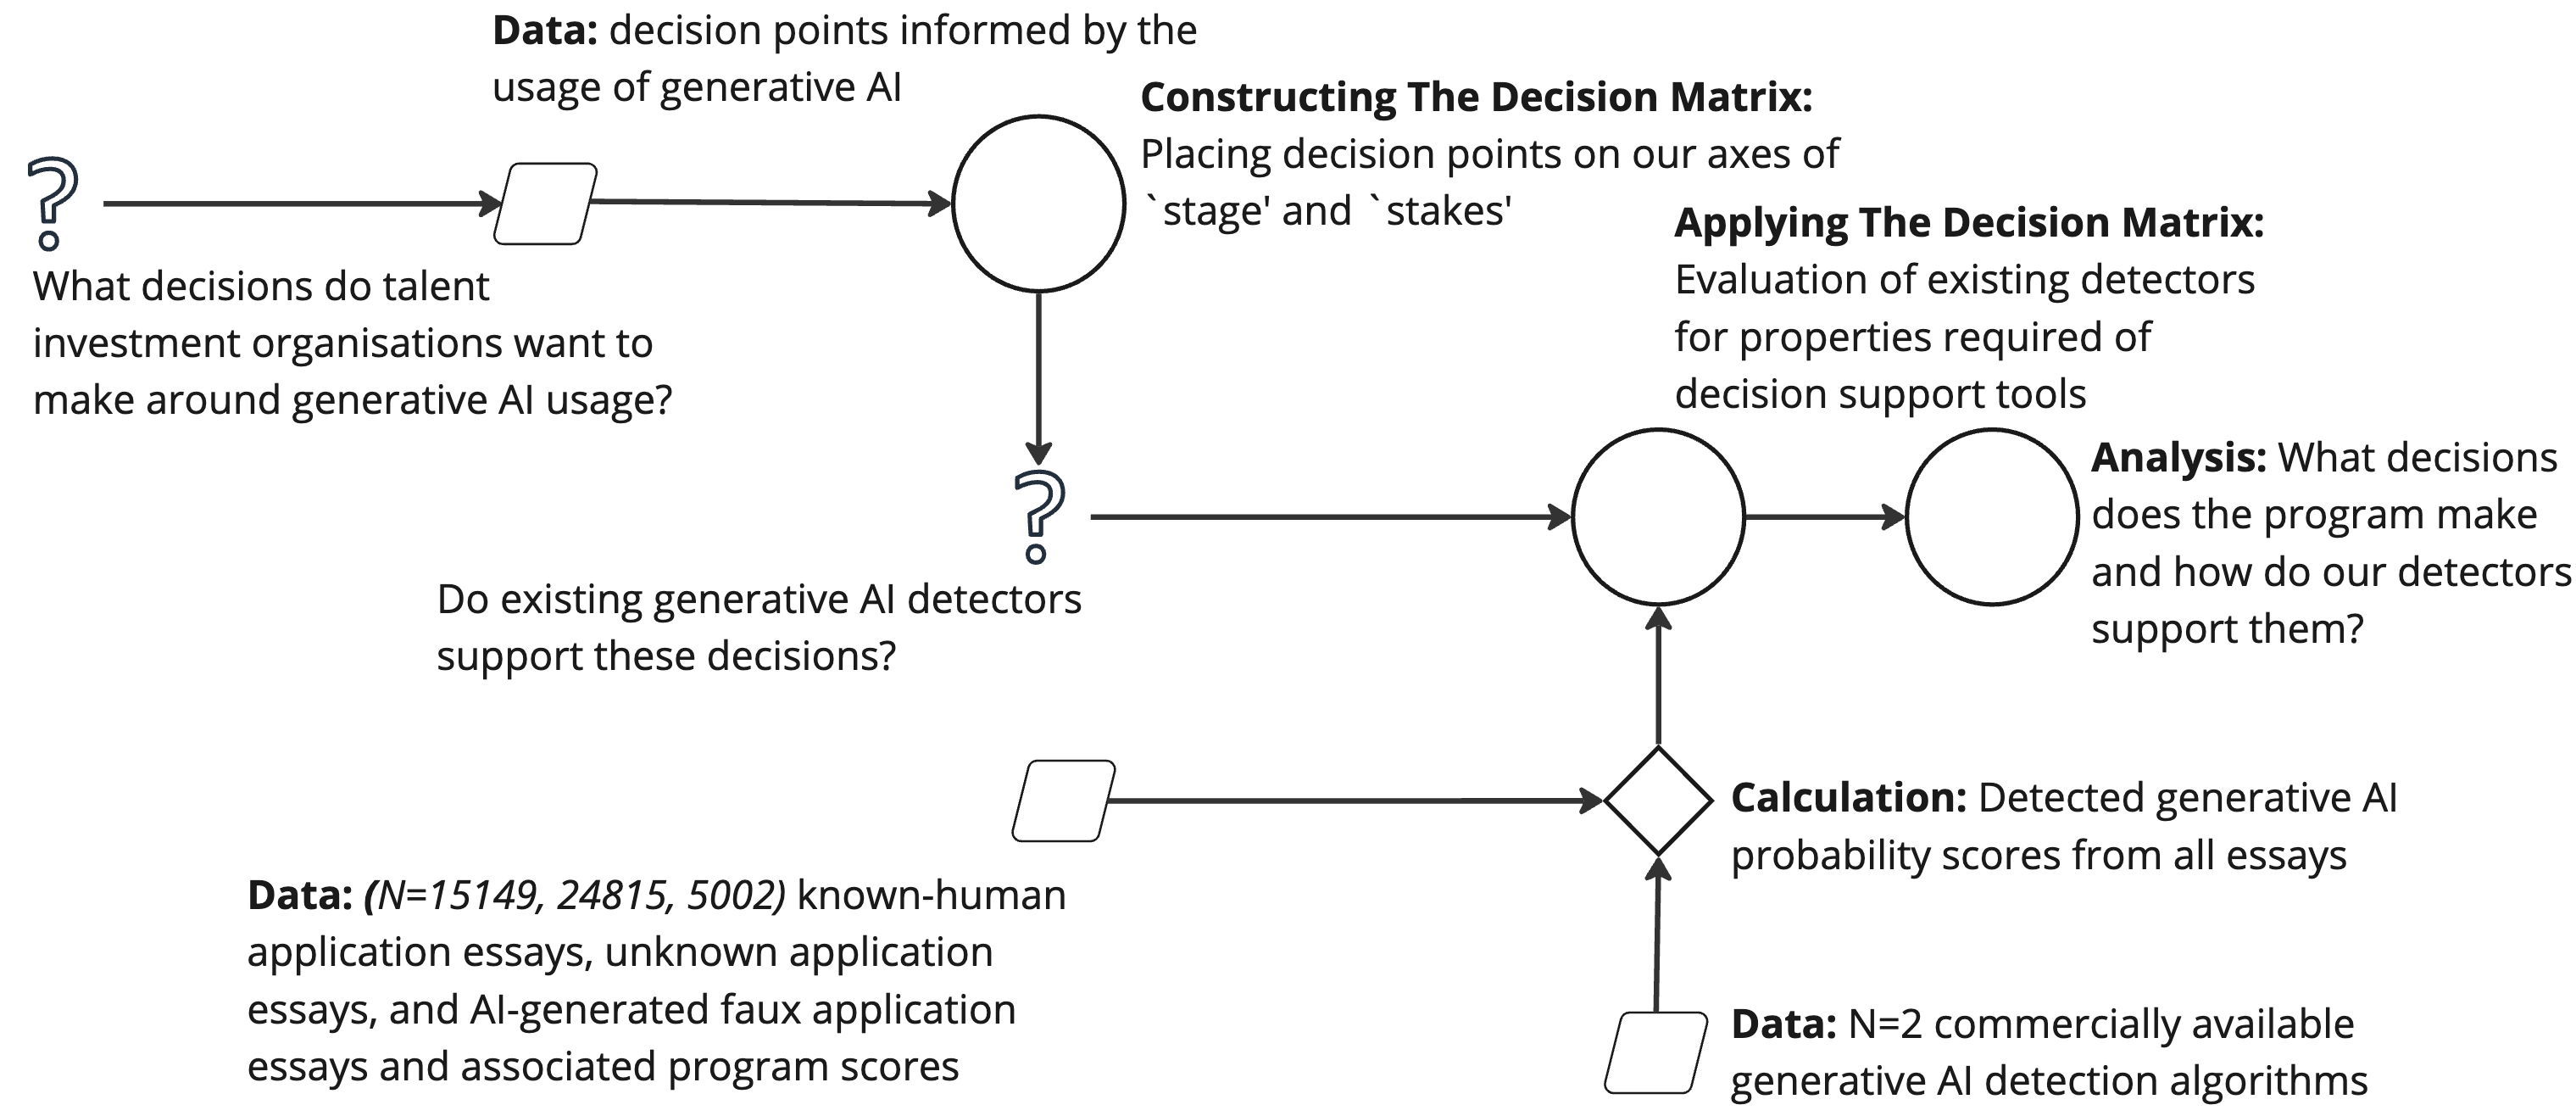
\includegraphics[width=\textwidth]{genai/study_flow.png}
  \caption{This figure describes the flow of our research.}
  \label{fig:flow}
\end{figure}

\section{Methodology and Action Research}\label{sec:embedded}
\subsection{What is Action Research?}\label{ssec:par}
Action Research (AR) is a research philosophy that emphasises ``research with, rather than on, people'' \cite{bradbury_action_2003}. Rather than one specific method, AR is best seen as a collection of related methods all embodying this ethos, usually with the goal of producing research contributions useful to the target group of people \cite{lu_organizing_2023}. Among these are semiotic inspection \cite{DeSouza_Leitão_2009,Alvarado_Waern_2018} and participatory design  (PD) \cite{braun_using_2006,Griffiths_Johnson_Hartley_2007,blythe2014research,Knapp_Zeratzky_Kowitz_2016}. AR is most often used in the context of social work, but can be applied across a variety of fields \cite{dombrowski_social_2016,lu_organizing_2023}. 

In education, AR is often used in a classroom setting \cite{Mertler_2019}. \textcite{venn-wycherley_realities_2024} argue that it is crucial in this setting to perform AR on both educators (teachers) and educatees (students), as failing to do so is liable to yield contributions useful to one group but not the other. While this holds for classroom settings, engagement across the stakeholder map is less feasible or desirable in scholarship selection. Unlike teacher and student, who share the common goal that the student learn, selector and applicant are at cross purposes: practitioners seek to choose the `best' cohort of applicants (although they often disagree on what constitutes `best'), while applicants seek to be included in the chosen cohort \cite{bergman2021seven}. Thus, when elucidating the interests and desires of one group, the other will merely act as noise. (E.g., applicants who use genAI to assist in writing their application will, of course, oppose using systems that monitor genAI usage to disqualify applicants.)

AR is comparatively new to HCI \cite{Hayes_2011,lu_organizing_2023}, but its methods and philosophies closely mirror longstanding pillars of HCI \cite{Hayes_2011}. Much like PD and other HCI methods, AR seeks to democratise the research and design processes; unlike PD, AR extends beyond building solutions democratically, and sees learning through action as the ultimate research contribution \cite{Hayes_2011}. For example, AR sees all parties Become: ``Co-investigators of, co-participants in, and co-subjects of...the project'' \cite{Hayes_2011}.  Thus, research questions are formulated by and with participants, actions and interventions are designed by and with participants, and results are found by and with participants \cite{Hayes_2011}.

\subsection{Our Action Research}
In many scholarship selection contexts, organisations typically select groups of talented young people based on applications consisting variously of: essays, videos, test scores, interviews, project results, group or individual activities, etc.. The organisation will begin by narrowing down the pool of candidates, often based primarily on test results, project results, or other easy-to-gather information. The organisation likely then compiles information from the application into short-form summaries of each applicant, complete with internally-generated scores, and often even a recommendation. This recommendation is then often reviewed by a selection committee, who craft a cohort from the recommended applicants.

We engage a scholarship and talent investment organisation in AR to investigate this selection context. In engaging this organisation in AR, several of the authors also functioned in supporting roles for the organisation's 2022 and 2023 selection cycles. In addition to working alongside the selection practitioners themselves, the authors were, at the time, a part of the scholarship organisation. Thus, throughout the paper, we refer to this organisation as our `partner organisation'. 

As with all AR, we first worked with participants (N=8; excludes authors) to identify research questions. We did this via a mixture of synchronous and asynchronous interactions. After this, we evaluated two genAI detectors, GPTZero and Originality.ai, according to our research questions. Finally, we implemented one genAI detector as an intervention. The flow of this study can be seen in Figure \ref{fig:flow}.

Before our study, we obtained consent from all 8 participants to be included. Applicant essay data was collected by our partner organisation, who obtained consent to use these essays (anonymously) for research purposes. Participants also gave consent to be recorded, and to have these recordings stored on a secure server. All recording, transcribing, and data analysis was conducted on secure servers. Ethics review was performed by University of Oxford's Central University Research Ethics Committee.

\subsection{Positionality}
Following \textcite{venn-wycherley_realities_2024}, we state researcher positionality here. The research team is comprised of five researchers split between the United States and United Kingdom; all researchers are men; four out of five researchers are ethnically White, while the fifth is South Asian; three researchers are affiliated with the University of Oxford and two are affiliated with Schmidt Futures.

\begin{table}[htbp]
  \centering
  \caption{Our partner program discussed a desire to make several decisions with regards to genAI. These decisions and the information desired to support them are detailed here. Though the program discussed disqualification, the program has no application guidelines surrounding the use of genAI and expressed no interest in disqualification. We include it here due to its ubiquity elsewhere in the literature \cite{liang_gpt_2023,mitchell_detectgpt_2023,tharindu_kumarage_stylometric_2023,kalpesh_krishna_paraphrasing_2023}.}
  \label{tab:decisions}
  \begin{tabular}{ p{0.2\linewidth}p{0.3\linewidth}p{0.5\linewidth}}
      \toprule
      Decision Point & Decision Description & Supporting Information \\
      \midrule
      \emph{Diligence} & The program makes holistic decisions about when and how to consider applicants. & Information about which essays (and which parts of essays) were written by genAI; information about whether the genAI-written passages are hallucinations. \\ 
      \emph{Partners} & The program must determine whether to continue channel partnerships, which encourage and support applicants. & Whether any channel partners' affiliated applicants use genAI disproportionately. \\
      \emph{Pipeline} & The program decides whether to modify their application material or process. & Information about usage of genAI throughout the application pipeline. \\
      \emph{Gameability} & The program decides how to modify their application material or process. & Information about the how AI-generated essays are scored under the current application process. \\
      \midrule
      \emph{Disqualification} & A program may decide to disqualify an applicant that violates their application guidelines. & Information about whether essays violate application guidelines around genAI usage. \\
      \bottomrule
  \end{tabular}
\end{table}


\section{Constructing the Decision Matrix}\label{ssec:poi}
We began from a starting point of ``What do we do about genAI?''. Literature about genAI elsewhere prompted early discussions to focus on: ``Can we determine whether an applicant used genAI to plagiarise?'' but quickly discarded this; the partner organisation had no application guidelines forbidding genAI usage, and hoped to accommodate ``innovative uses of this powerful technology'' in their selection process. From there, we quickly moved to ``What decisions do talent investment organisations want to make around generative AI usage?''. We then sought out other decisions the program wished to make in response to genAI. Ultimately, we identified the decision points in Table \ref{tab:decisions}; our final research question, then, is ``Do existing generative AI detectors support these decisions?''.

Notably, the decision to disqualify applicants for using genAI (\emph{Disqualification}) appears several times in the literature surrounding potential use cases for detectors \cite{gptzero_gptzero_2023,kalpesh_krishna_paraphrasing_2023}. Thus, despite our partner organisation's dismissal, we list it alongside the different decisions discussed in Table \ref{tab:decisions}.

\begin{figure}[htbp]
  \centering
  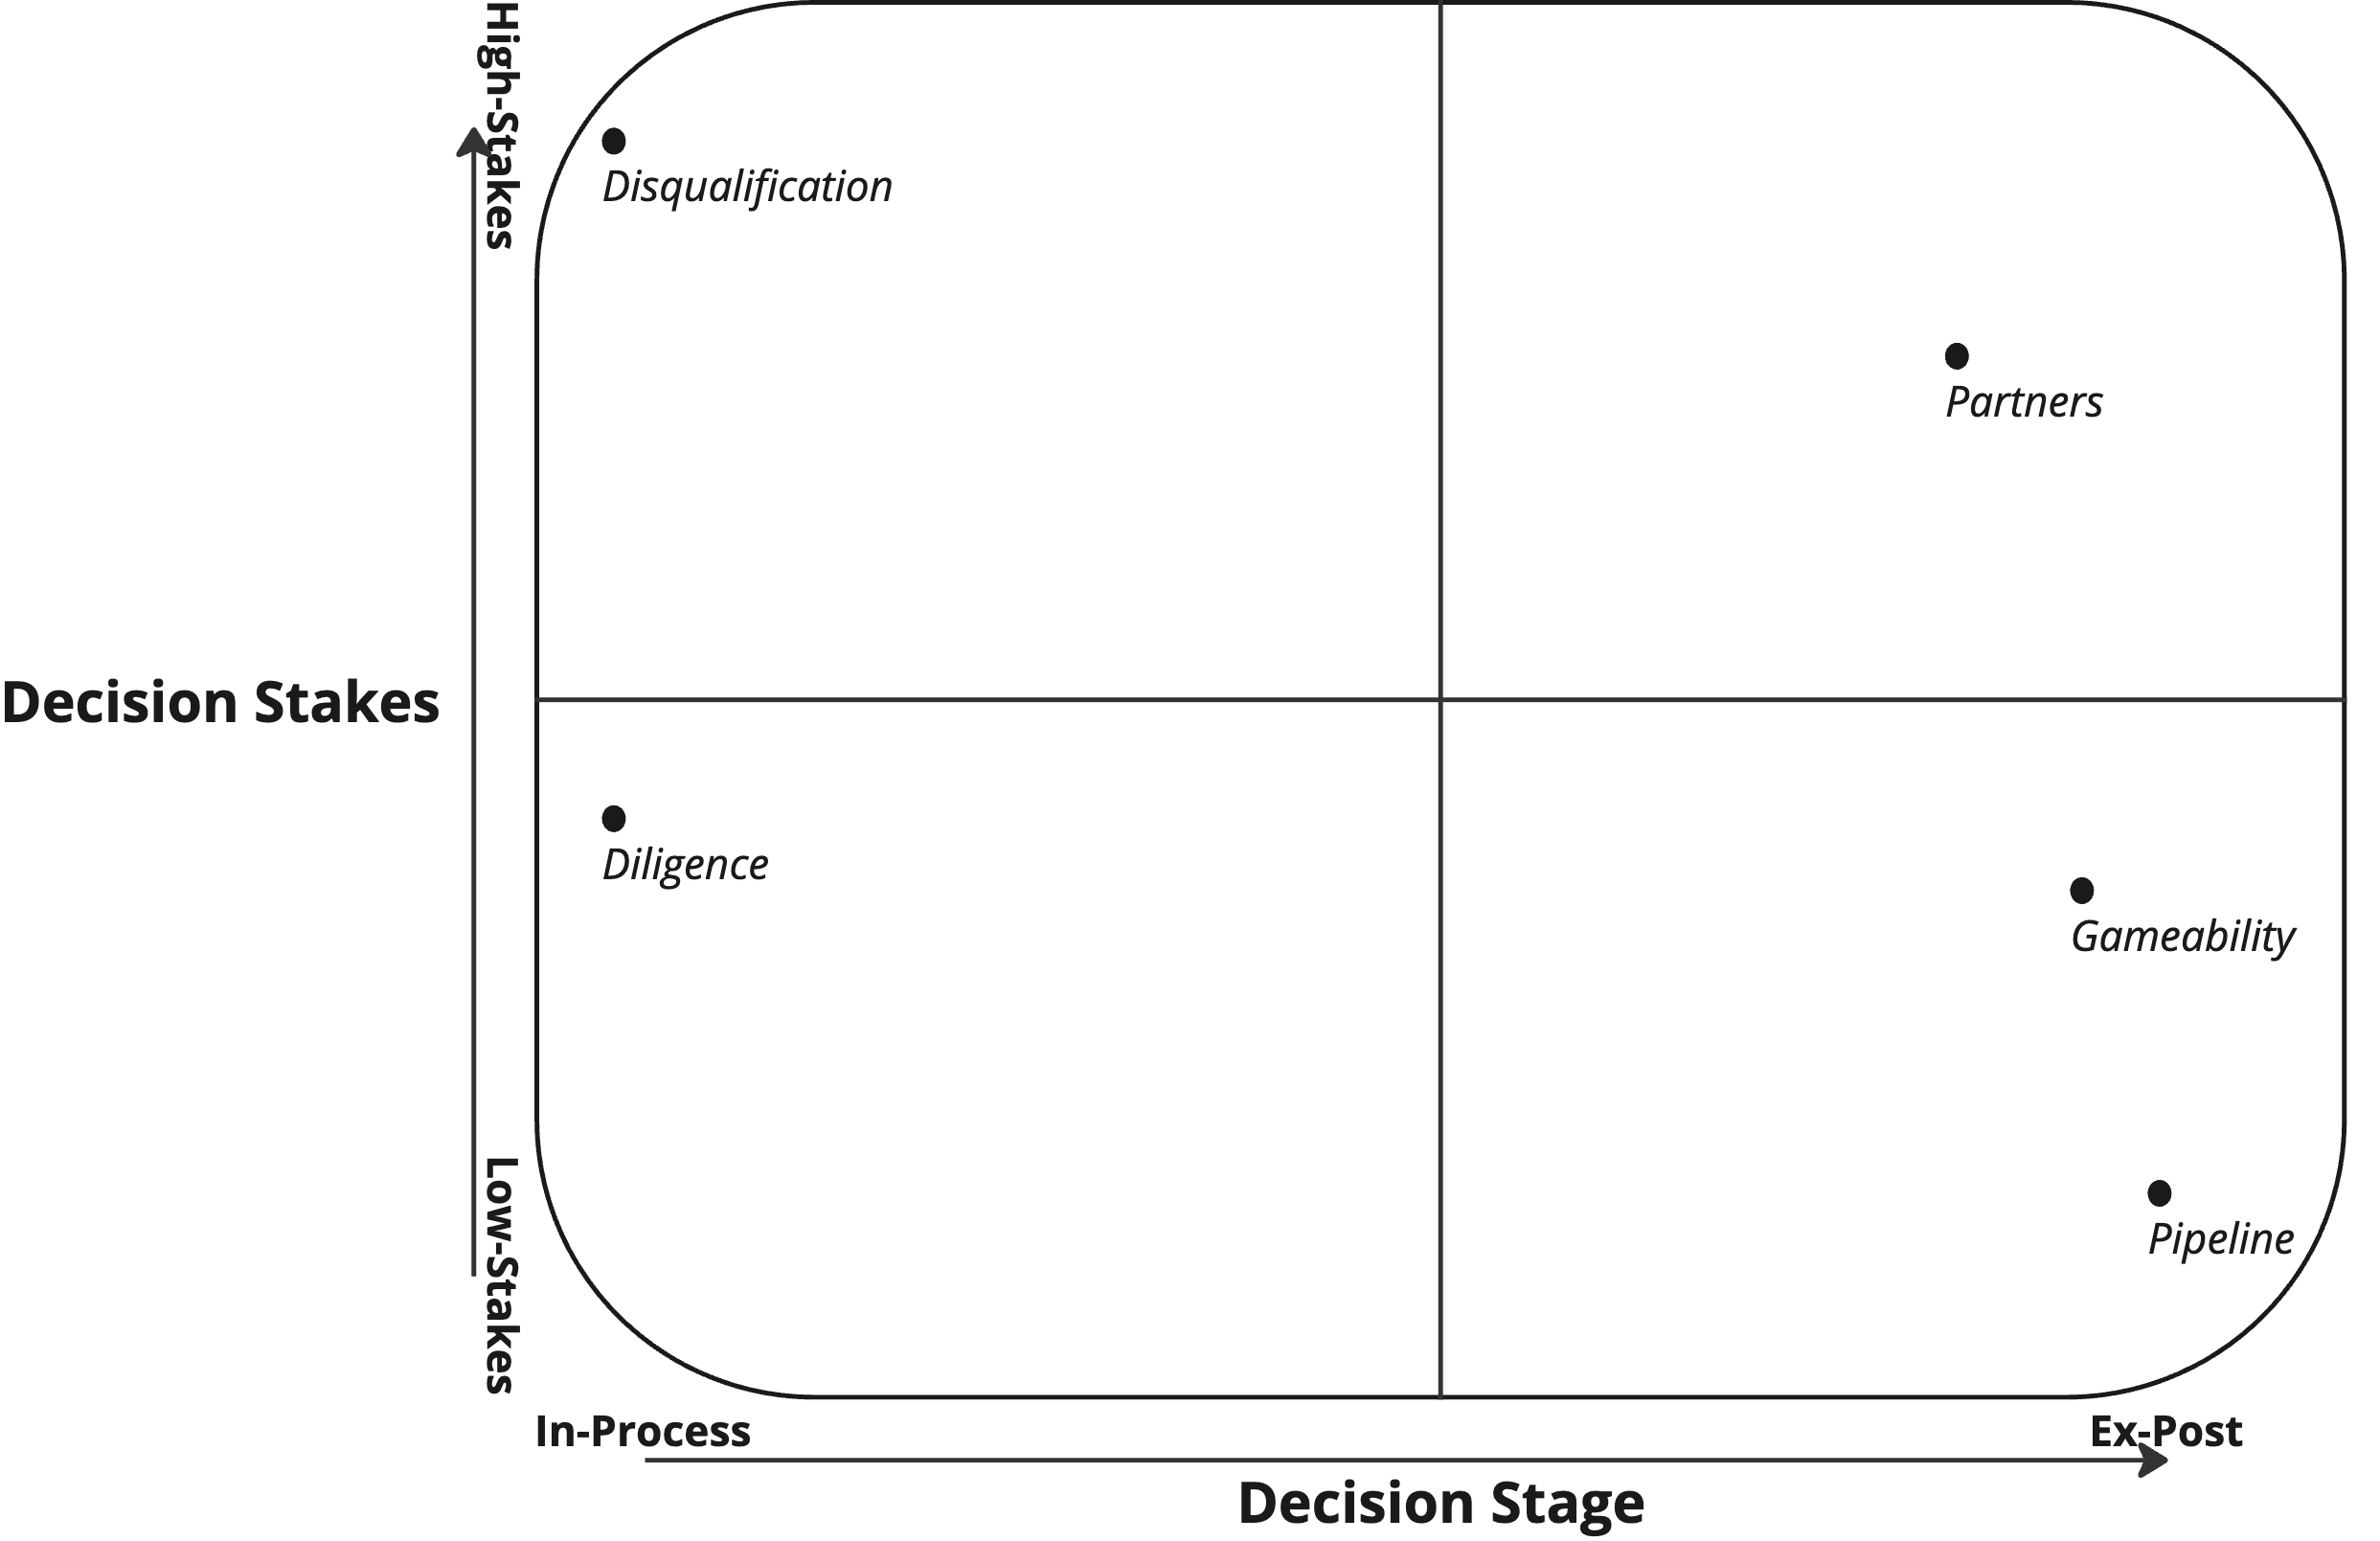
\includegraphics[width=0.8\textwidth]{genai/decision_matrix.png}
  \caption{This figure places the decisions from Table \ref{tab:decisions} on the Decision Matrix, with axes of `stage' and `stakes'.}
  \label{fig:decision_matrix}
\end{figure}

In conversation with practitioners in our partner program, we isolated two `axes' on which the decision points exist: stage and stakes. Decision stages vary from entirely in-process (`primary' decisions during the selection process) to entirely ex-post (`secondary' decisions about future selection processes). Meanwhile, decision stakes vary from very low (e.g., a due-diligence decision to investigate further) to very high (e.g., a decision to disqualify an applicant). Figure \ref{fig:decision_matrix} uses these axes to categorise the decisions in Table \ref{tab:decisions}.

We also work with practitioners to determine what type of properties a detection score should have to support each decision. For example, a disqualification decision may have stricter requirements than a diligence one. We lay out these desiderata on the same axes as Figure \ref{fig:decision_matrix} in Figure \ref{fig:desiderata_matrix}. 

\begin{figure}[htbp]
  \centering
  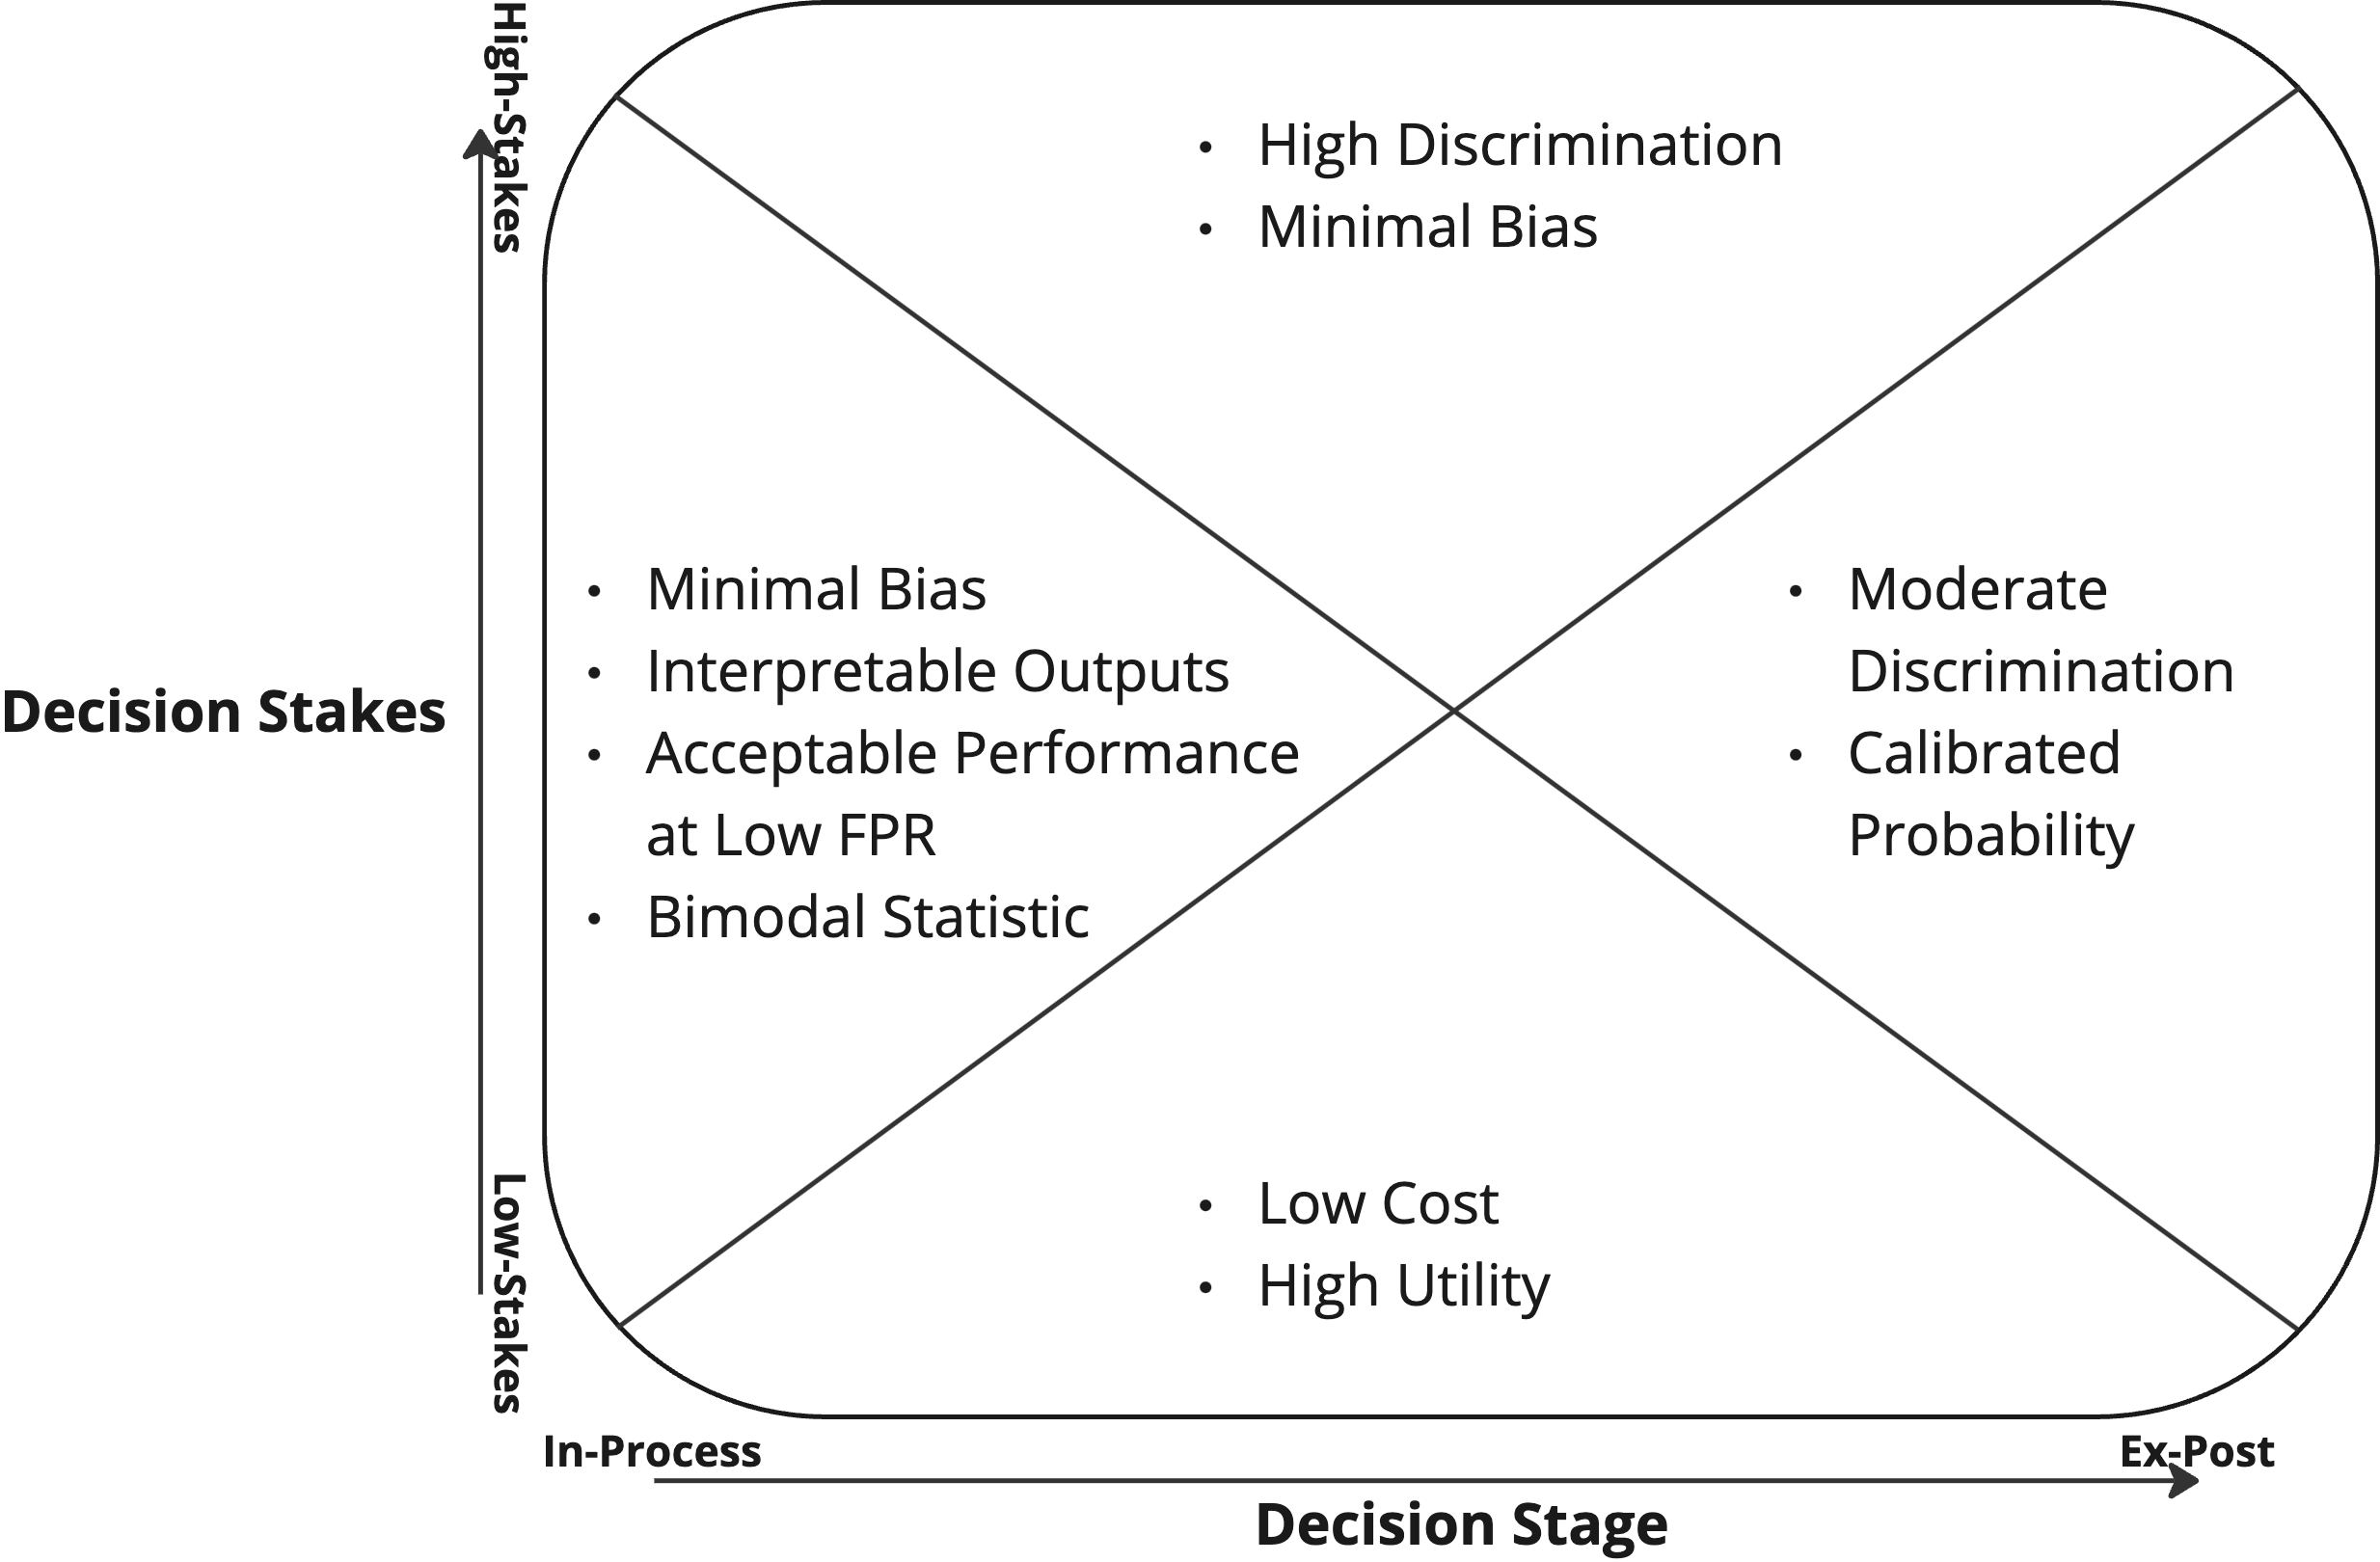
\includegraphics[width=0.8\textwidth]{genai/desiderata_matrix.png}
  \caption{This figure places uses our Decision Matrix to understand properties of genAI detectors required (or, in the case of low-stakes decisions, desired) to support each decision.}
  \label{fig:desiderata_matrix}
\end{figure}

\section{Applying the Decision Matrix}\label{sec:data}
\subsection{Evaluating for Decisions}
We seek to evaluate genAI detection software for its suitability in supporting decisions across the Decision Matrix in Figure \ref{fig:decision_matrix}. To do this, we first evaluate detectors on the properties outlined in Figure \ref{fig:desiderata_matrix}; if a detector has the properties outlined in both low-stakes and ex-post decisions, it is likely to be useful in supporting decisions from this quadrant. However, although our partner program indicated that these properties are necessary, we still seek to test their sufficiency. Thus, where the desiderata are satisfied, we apply the detectors to specific decisions from Figure \ref{fig:decision_matrix}. In particular, we select one decision from each quadrant (unless all detectors are deemed to lack the properties required for decision support in that quadrant). Finally, in case multiple detectors have sufficient properties, we compare detectors directly to make a recommendation about which method practitioners should use for these use cases.

\subsection{Data}
\subsubsection{Applicant Data}\label{sssec:applicant_data}
We use data from two of our partner program's application cycles, which we term Cycle 2022 and Cycle 2023.

Applications for Cycle 2022 were due in early 2022, well before ChatGPT's public release, so we assume that these submissions were written without the use of genAI \cite{openai_gpt-4_2023}. Applications for Cycle 2023 were due in early 2023, so genAI tools were widely available and AI detection tools were already emerging \cite{kirchner_new_2023,gptzero_gptzero_2023,liu_deid-gpt_2023}; we thus make no such assumption for these applications.\footnote{A number of avoidance detection strategies (e.g., paraphrasers) have been proven to severely hamper state-of-the-art detection \cite{kalpesh_krishna_paraphrasing_2023}. However, as of the 2023 deadline, the efficacy of these detection avoidance strategies was not well-known. Thus, we assume these strategies were not widely employed.}

\begin{table}[htbp]
    \centering
    \caption{This table shows the total number of submitted essays evaluated across years and demographic groups.}
    \label{tab:demo_counts}
    \begin{tabular}{ l r r }
        \toprule
        Demographic Group & 2022 Essays & 2023 Essays \\
        \midrule
        Male & $6,475$  & $11,080$ \\
        Female & $8,710$  & $13,380$ \\
        Other & $176$ & $355$ \\
        \midrule
        Caribbean & $128$ & $75$ \\
        East and Southeast Asia & $1,332$ & $395$ \\
        Core Anglosphere & $522$ & $1,865$ \\
        Eastern Europe / Central Asia & $85$ & $705$ \\
        South Asia & $2,130$ & $2,560$\\
        Latin America & $709$ & $2,855$ \\
        Middle East / North Africa & $1,363$ & $4,100$ \\
        Sub-Saharan Africa & $8,972$& $8,375$\\
        Western Europe & $59$ & $560$ \\
        Pacific Islands & $5$& $0$ \\
        \midrule
        Total & $15,149$ & $24,815$ \\
        \bottomrule
    \end{tabular}
\end{table}

Each applicant submitted essays in response to five prompts. These prompts are not described in more detail to preserve our partner organisation's anonymity. Applicants in both cycles provided information on their background, including gender identity and countries of citizenship. 

Applicants were asked their gender identity and given options including `male', `female', `non-binary', `other', and `prefer not to say'. The program uses all categories. However, the vast majority selected `male' or `female', so, in order to avoid spurious results from small samples, we group `non-binary' and `prefer not to say' under `other' for this analysis. 

Similarly, applicants reported their primary, secondary, and tertiary nationalities (where they exist). The program uses only primary nationalities in this context, and has, throughout the 2022 and 2023 application cycles, grouped applicants in various ways. The program uses the given `semi-regional' groupings to capture relevant similarities between nationalities (e.g., while `Core Anglosphere' is not a distinct geographic region, applicants from Core Anglosphere countries tend to speak English as their first language, come from similar school systems, and share similar facets of culture). These regional groupings are the program's. At the program's request, we do not share specific country-to-region codings.

Table \ref{tab:demo_counts} describes the analytic sample of essays by these demographic dimensions for each cycle. 

\subsubsection{Synthetic Data}\label{sssec:chatgpt}
To obtain a set of known AI-generated essays, we generate $5,002$ synthetic essays using OpenAI's ChatGPT API and Cycle 2022 prompts. These sit alongside our $15,149$ human-written, applicant-submitted Cycle 2022 essays and form our Cycle 2022 corpus. In contrast, our Cycle 2023 corpus consists entirely of applicant-submitted essays, though it is unknown how many of these are AI-generated. Our entire corpus is detailed in Table \ref{tab:cycle_counts}.

\begin{table}[htbp]
  \centering
  \caption{This table shows the total number of (submitted and generated) essays. The top row, Cycle 2022 submissions, is assumed to be human-written, as the Cycle 2022 submission deadline predates the release of ChatGPT. The second row lists essays generated by the authors in response to the Cycle 2022 prompts. The third row lists submitted essays of unknown providence from the 2023 application cycle.}
  \label{tab:cycle_counts}
  \begin{tabular}{ l r }
      \toprule
      Source  & Essays \\
      \midrule
      Cycle 2022 Submissions (Assumed Not AI) & $15,149$ \\
      ChatGPT Responses to Cycle 2022 Prompts & $5,002$ \\
      Cycle 2023 Submissions (Potentially AI) & $24,815$ \\
      \bottomrule
  \end{tabular}
\end{table}

All of our synthetic essays were generated via OpenAI's ChatGPT API using GPT-3.5 \cite{brown_language_2020}. More detail on our prompts can be found in Appendix \ref{app:prompt}.

\subsubsection{Detectors}\label{sssec:detectors}
Despite the myriad of available genAI detection tools, standardised comparisons of detectors are few and far between, but what benchmarks do exist list similar models as leaders in accuracy across standard FPR thresholds. \textcite{dugan_raid_2024} introduce RAID, a standardised genAI detection benchmark, and apply it to twelve popular models. Their results are mixed, but demonstrate a clear advantage for three detectors: the open-source Binocular model, and the commercial GPTZero and Originality.ai models \cite{dugan_raid_2024}. \textcite{verma_ghostbuster_2023} compare GPTZero, DetectGPT, two baselines, and their own model, Ghostbuster. Their results are similarly mixed but, in a variety of scenarios, GPTZero or Ghostbuster variously perform best \cite{verma_ghostbuster_2023} . Our partner organisation reached out to both GPTZero and Originlity.ai, and both offered us access to their models for research purposes.

To calculate scores, we use the API under default settings for both GPTZero and Originality.ai. Note that we calculated our GPTZero-based detection scores in early 2023, while the Originality.ai scores were calculated more recently in mid 2024. Thus, it is possible that a more recent version of GPTZero's model has since been made available; our results apply only to the 2023 version we used. This yielded various statistics from each detector for each essay, but we are primarily interested in the overall likelihood statistic from each.

\begin{figure}[htb]
  \centering
  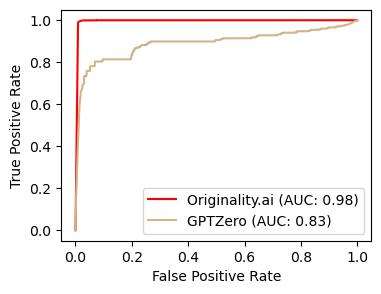
\includegraphics[width=0.4\textwidth]{genai/roc_curve.jpg}
  \caption{This Receiver Operating Characteristic (ROC) curve shows the performance of each detector on our data of known providence (Cycle 2022 submissions and ChatGPT responses to Cycle 2022 prompts). While GPTZero's ROC curve has a moderate area under the curve (AUC), Originality.ai's ROC curve has a very high AUC.}
  \label{fig:roc_auc}
\end{figure}

\subsection{Results}
\subsubsection{Both Detectors Possess the Properties Desired for Low-Stakes Decision Support}
We identified no properties required to support low-stakes decisions, but list several desiderata that we consider more a matter of utility than of necessity. In particular, detectors should have:

\begin{enumerate}
    \item Low cost
    \item High utility
\end{enumerate}

We measure cost as the price per essay evaluated at the highest tier of subscription service available from each detector in Table \ref{tab:detector_cost}. We measure utility according to ROC AUC.

Table \ref{tab:detector_cost} shows that both detectors have low cost, with GPTZero having slightly lower cost.\footnote{As we used both detectors for research purposes, we reached out to the companies involved and were given research access. These cost estimates are based not on our access, but on public information assuming the highest tier of subscription service available from each detector.}

Figure \ref{fig:roc_auc} demonstrates high utility from both detectors, though Originality.ai has a higher ROC AUC than GPTZero. Overall, both detectors satisfy the desiderata specific to low-stakes decisions.

\begin{table}[htbp]
  \centering
  \caption{This table displays estimated per-essay costs of each detector; both detectors are deemed sufficiently cost-effective.}
  \label{tab:detector_cost}
  \begin{tabular}{l r}
      \toprule
      Detector & Cost per Essay \\
      \midrule
      GPTZero & $\$0.023$ \\
      Originality.ai & $\$0.06$\\
      \bottomrule\\
  \end{tabular}
\end{table}

\subsubsection{GPTZero Possesses the Properties Required for High-Stakes Decision Support}\label{sssec:highstakes}
We identified two properties required to support high-stakes decisions. Detectors should have:

\begin{enumerate}
    \item High discrimination
    \item Low bias
\end{enumerate}

We measure discrimination as by whether the detector clearly discriminates positive and negative cases (see Table \ref{tab:detector_cost}). We measure bias as the difference in FPR between demographic groups.

\begin{figure}[htb]
  \centering
  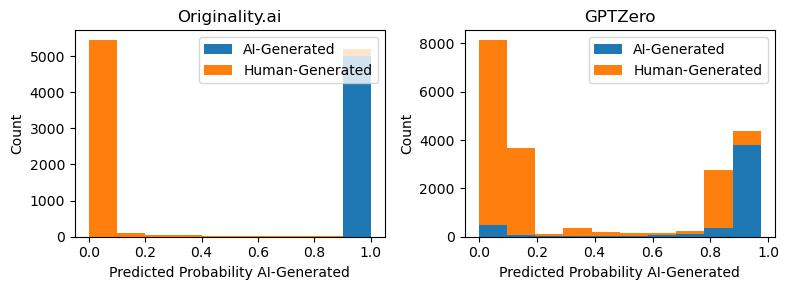
\includegraphics[width=0.8\textwidth]{genai/histogram.jpg}
  \caption{These histograms demonstrate the high bimodality and predictive discrimination of both detectors' outputs.}
  \label{fig:histogram}
\end{figure}

As can be seen in Figure \ref{fig:histogram}, both detectors' outputs are close to either 0 or 1, though Originality.ai has far higher discrimination than GPTZero. This is reflected in the confusion matrices in Figure \ref{fig:confusion}. As can be seen, both output statistics discriminate well between positive and negative cases. However, while GPTZero clearly discriminates between positive and negatives, Figure \ref{fig:confusion} shows that Originality.ai has lower error of both types.

\begin{figure}[htb]
  \centering
  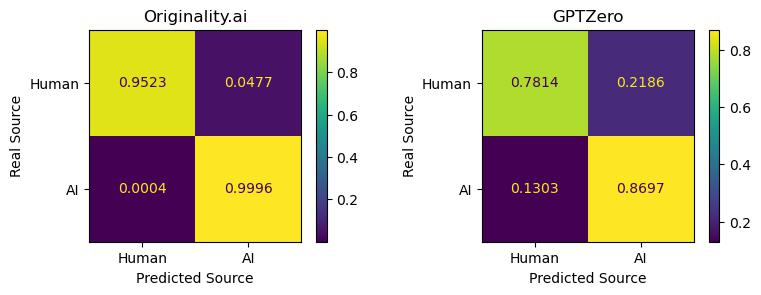
\includegraphics[width=0.8\textwidth]{genai/confusion.jpg}
  \caption{These confusion matrices again demonstrate the high predictive discriminative capabilities of both detectors' outputs.}
  \label{fig:confusion}
\end{figure}

We see bias in both statistics in Table \ref{tab:demo_means_c2}, as the FPRs (average detection statistic on known-human essays) differ by demographic in both cases. Interestingly, though GPTZero has much higher false positive rates in all cases, these rates differ less by demographic than those of Originality.ai (this can be seen in the lower ANOVA statistic). This results in us observing Originality.ai ANOVA statistics $2.75$ and $3.40$ greater than GPTZero ones, respectively. This is, practically, the difference between minor between-group variance and measurable and harmful bias. For this reason, although both detectors have bias, we believe that GPTZero's bias does not render it unsuitable for ex-post decisions across our applicant pool, while Originality.ai's does.\footnote{Note that, in the case of Originality.ai, this appears to be driven by disparate performance across regions (and the ``Other'' gender category). Organisations with more regionally homogeneous applicants may wish to re-analyse Originality.ai's biases across their relevant demographics.} In this case, our partner organisation saw the high risk of false positive from the GPTZero statistic as sub-optimal, but deemed the bias demonstrated by Originality.ai, particularly across different regions, untenable.

\begin{table*}[htbp]
  \centering
  \caption{This table displays FPRs for both detectors split by applicant demographics and compared by ANOVA in the (human-written) Cycle 2022 submissions. Differences in FPR here can be interpreted as bias: both detectors display a bias, but Originality.ai displays a far higher bias than GPTZero.}
  \label{tab:demo_means_c2}
  \begin{tabular}{l r r}
      \toprule
      Demographic Group & GPTZero & Originality.ai \\
      \midrule
      Male                    & $0.23$ & $0.06$ \\
      Female                  & $0.23$ & $0.07$ \\
      Other                   & $0.21$ & $0.16$ \\
      ANOVA Statistic         & $\mathbf{0.11}$ & $\mathbf{2.86}$ \\
      \midrule
      Caribbean               & $0.17$ & $0.00$ \\
      East and Southeast Asia     & $0.24$ & $0.06$ \\
      Core Anglosphere               & $0.21$ & $0.17$ \\
      Eastern Europe / Central Asia    & $0.23$ & $0.17$ \\
      South Asia     & $0.22$ & $0.07$ \\
      Latin America           & $0.21$ & $0.02$ \\
      Middle East / North Africa   & $0.25$ & $0.05$ \\
      Sub-Saharan Africa      & $0.23$ & $0.06$ \\
      Western Europe            & $0.20$ & $0.00$ \\
      Pacific Islands         & $0.04$ & $0.00$ \\
      ANOVA Statistic         & $\mathbf{0.57}$ & $\mathbf{3.97}$ \\
      \midrule
      All Submissions         & $0.23$ & $0.05$ \\
      \bottomrule
  \end{tabular}
\end{table*}

\subsubsection{Both Detectors Possess the Properties Required for Ex-Post Decision Support}
We identified two properties required to support ex-post decisions. Detectors should have:

\begin{enumerate}
    \item Moderate Discrimination
    \item Calibrated Probability\footnote{Calibrated statistics are ones whose distributions are probability-like in expectation.}
\end{enumerate}

We measure discrimination as in Section \ref{sssec:highstakes}. We measure statistic calibration using calibration curves in Figure \ref{fig:calibration}.

We have already determined in Figure \ref{fig:roc_auc} that Originality.ai has particularly high predictive discrimination, while GPTZero has moderate predictive discrimination suitable for ex-post analyses.

\begin{figure}[htb]
  \centering
  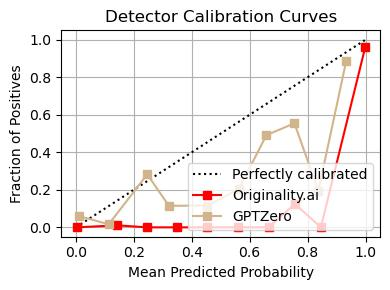
\includegraphics[width=0.4\textwidth]{genai/calibration.jpg}
  \caption{These calibration curves demonstrate the bimodality of both detectors' outputs. As can be seen, both output statistics fall far below the calibration curve; these output statistics are not calibrated on our data.}
  \label{fig:calibration}
\end{figure}

In aggregate analyses, we desire to reason about the probability that a particular essay was generated by AI ($P(AI)$), or even the expected number of AI-generated essays in a given group ($E(P(AI))$). This yields convenient general properties, e.g., $E(P(AI))$ is just the mean $P(AI)$ within a given group. Figure \ref{fig:calibration} provides a calibration curve for both detectors, and demonstrates a comparative lack of calibration in both cases. In both cases, output statistics fall far below the calibration curve, indicating a bias towards extrema. In effect, this entails that we should not treat these output statistics like probabilities. However, so long as we have a large provenance of labelled data (which we do in the form of $15,149$ applicant-submitted and $5,002$ ChatGPT-generated Cycle 2022 essays), we can calibrate an uncalibrated statistic to achieve a more probability-like output. In our case, we calibrate our statistics on our data by applying a monotonic transformation to ensure that, within any subset of our body of essays, the mean predicted probability aligns with the fraction of positive cases.

Thus, we conclude that, post-calibration, both detectors possess the properties of probabilities that we would require for use in ex-post analyses. We caution other organisations against using these detectors for these purposes without first calibrating their output statistics on data of known provenance.

\subsubsection{Neither Detector Possesses the Properties Required for In-Process Decision Support}
We identified four properties required to support in-process decisions. Detectors should have:

\begin{enumerate}
    \item Minimal Bias
    \item Interpretable Outputs
    \item Acceptable Performance at Low FPR
    \item Bimodal Statistic
\end{enumerate}

We measure bias as in Section \ref{sssec:highstakes}. We reason about model interpretability. We measure acceptable performance at low FPR based on TPR rates at an FPR of $\%1$. We measure bimodality using the histogram in Figure \ref{fig:histogram} and the calibration curve in Figure \ref{fig:calibration}.

Recall that, in Table \ref{tab:demo_means_c2}, we observe bias in both outputs, and conclude that, while GPTZero is sufficiently balanced across demographic groups, Originality.ai's outputs display too much regional bias for our purposes. 

We also note that GPTZero provides interpretability in the form of local-level scores that might direct a human overseer's attention to particularly problematic phrases or sentences. Originality.ai, in contrast, only provides a single overall statistic. 

Figure \ref{fig:histogram} demonstrates the bi-modality of both detectors. Though it is clear that Originality.ai's output is more bimodal, we consider both detectors sufficiently bimodal for our purposes.

\begin{table*}[htbp]
  \centering
  \caption{This table displays TPRs at $\%1$ FPR.}
  \label{tab:tprs}
  \begin{tabular}{l r r}
      \toprule
      Detector & TPR \\
      \midrule
      GPTZero & $\%36.0$ \\
      Originality.ai & $\%98.9$ \\
      \bottomrule
  \end{tabular}
\end{table*}

Finally, to analyse performance at low FPR, our organisation set the acceptable FPR at $\%1$. We see TPR of $\%36.0$ for GPTZero and $\%98.9$ for Originality.ai in Table \ref{tab:tprs}. While GPTZero's output statistics are interpretable and display limited bias, it fails at low FPR rates.

\begin{figure}[htbp]
  \centering
  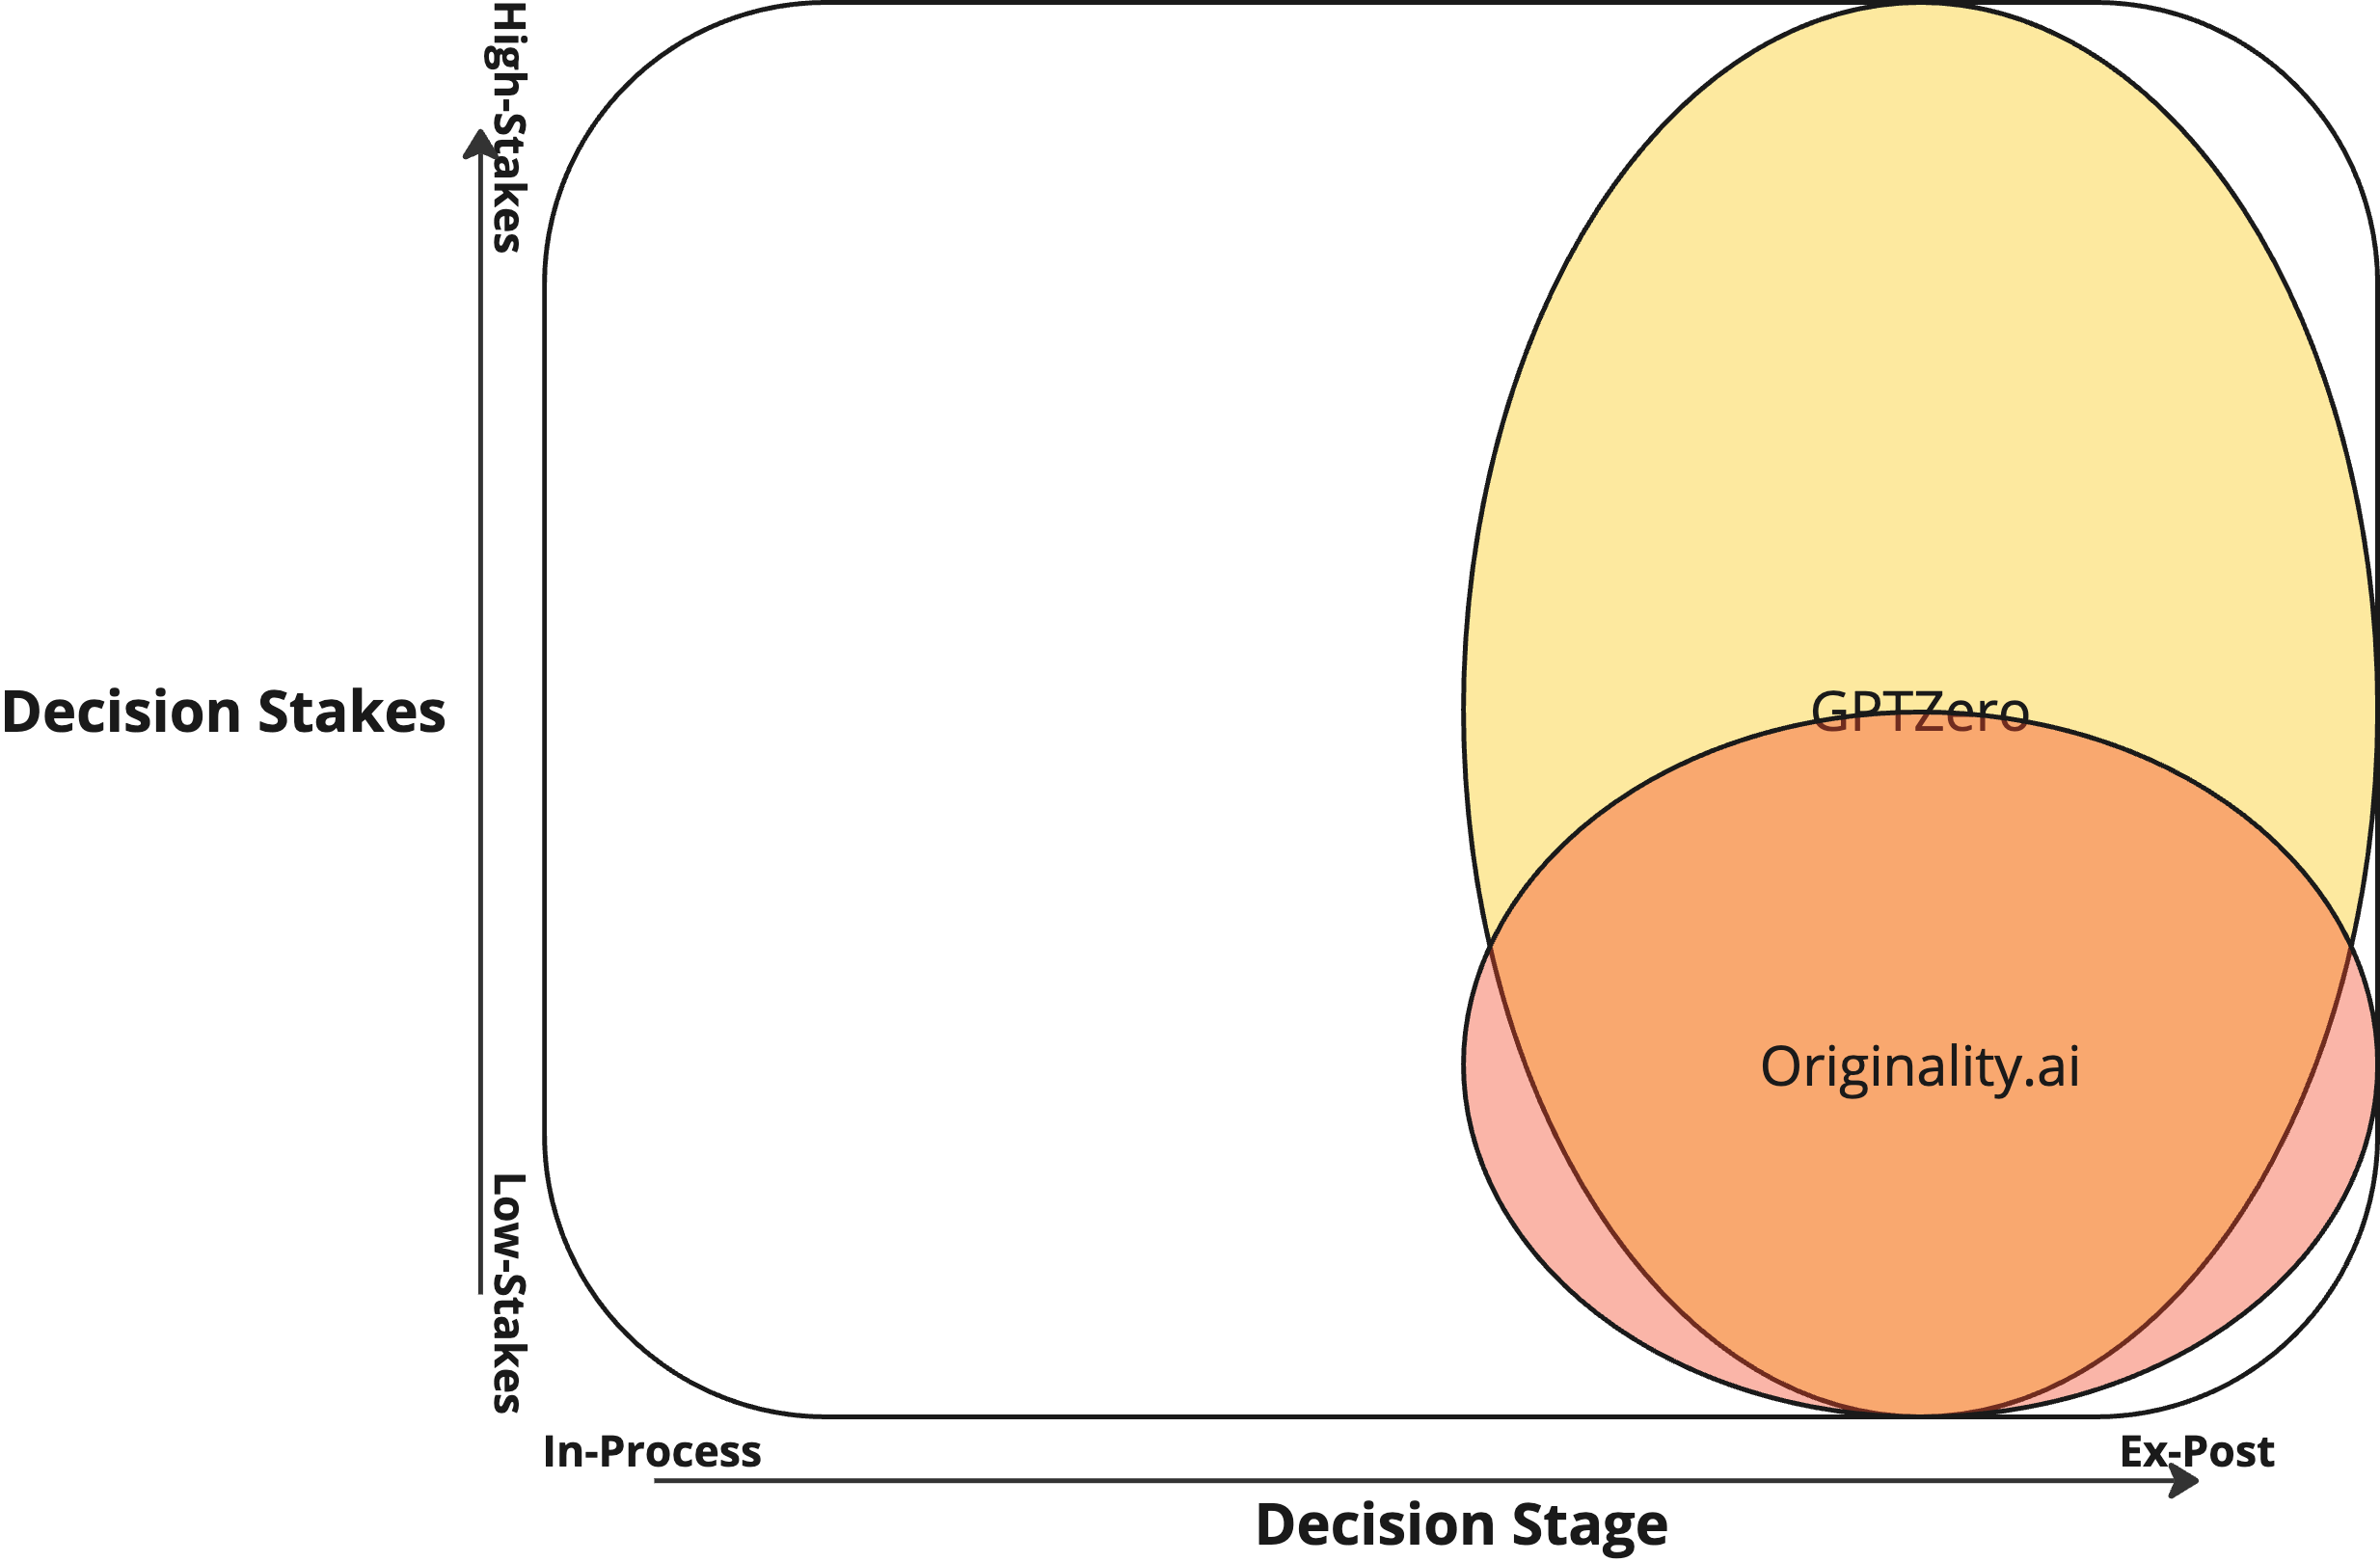
\includegraphics[width=0.8\textwidth]{genai/satisfaction_matrix.png}
  \caption{This figure demonstrates the results of our application of the Decision Matrix, marking the use cases we consider suited for each detector.}
  \label{fig:satisfaction_matrix}
\end{figure}

\section{Analysis of \emph{Pipeline} and \emph{Partners}}\label{ssec:decisions}

\subsection{Low-Stakes Ex-Post: Analysing Overall GenAI Usage in the 2023 Application Cycle (\emph{Pipeline})}
We focus our subsequent analysis primarily on the potential use of genAI by applicants in Cycle 2023. Seeking to avoid the disproportionate effects induced by GPTZero's heterogeneous biases (see Table \ref{tab:demo_means_c2}), we focus primarily on within-group changes. We note here that the mean probability of an essay being AI-generated within a corpus is exactly the expected proportion of AI-generated content within that corpus. Thus, we test for changes in mean $P(AI)$. As we have previously confirmed GPTZero is suitable for these analyses, we use our calibrated GPTZero score going forward. Table \ref{tab:demo_means_c23} presents mean $P(AI)$ for 2023 (column 3) and 2022 (column 5), as well as test statistics of whether there is a difference in means (columns 6 and 7). 

\begin{table*}[htbp]
  \centering
  \caption{These t-tests comparing $\widehat{E(P(AI))}$ across the 2022 and 2023 application cycles for each demographic reveal several changes by demographic, but only a small overall increase in AI-generated content.}
  \label{tab:demo_means_c23}
  \begin{tabular}{l r r r r}
      \toprule
      & Cycle 2022 & Cycle 2023 & \multicolumn{2}{c}{Inter-Cycle $\Delta$} \\
      Demographic Group & $\widehat{E(P(AI))}$ & $\widehat{E(P(AI))}$ & Test Statistic & p Value \\
      \midrule
      Male    & $0.09$ & $0.11$ & $\mathbf{8.63}$ & $\mathbf{<0.01}$ \\
      Female  & $0.11$ & $0.11$ & $-0.40$ & $0.69$ \\
      Other   & $0.14$ & $0.12$ & $-1.10$ & $0.27$ \\
      \midrule
      Caribbean               & $0.17$ & $0.15$ & $-0.47$ & $0.64$ \\
      East and Southeast Asia     & $0.13$ & $0.13$ & $0.74$ & $0.46$ \\
      Core Anglosphere               & $0.21$ & $0.14$ & $\mathbf{-5.86}$ & $\mathbf{<0.01}$ \\
      Eastern Europe / Central Asia     & $0.13$ & $0.15$ & $0.59$ & $0.56$ \\
      South Asia     & $0.08$ & $0.09$ & $\mathbf{2.65}$ & $\mathbf{0.01}$ \\
      Latin America           & $0.13$ & $0.09$ & $-1.44$ & $0.15$ \\
      Middle East / North Africa   & $0.11$ & $0.12$ & $1.67$ & $0.09$ \\
      Sub-Saharan Africa      & $0.09$ & $0.09$ & $\mathbf{2.15}$ & $\mathbf{0.03}$ \\
      Western Europe            & $0.20$ & $0.12$ & $\mathbf{-2.75}$ & $\mathbf{0.01}$ \\
      Pacific Islands         & $0.04$ & N/A      &  &  \\
      \midrule
      All Submissions         &$0.10$ & $0.11$ &  &  \\
      \bottomrule
  \end{tabular}
\end{table*}

We find statistically significant increases in the $P(AI)$ for only two overlapping subgroups: male applicants and applicants from the Indian subcontinent. In both cases the magnitude of the increase is small, suggesting that at least in Cycle 2023, the use of genAI was limited. However, other findings preclude interpreting this change as a direct measure of increased genAI use. In two regions, the Core Anglosphere and Western Europe, we found a statistically significant decrease in the calibrated estimated probability that essays were completely AI generated. Since we can assume very few if any applicants in Cycle 2022 had access to genAI, this cannot be interpreted as a decrease in AI use. It may be that both regions' high average scores in 2022 were a fluke of the cohort, and that these regions reverted to the mean in 2023. Alternatively, it is possible that, in these regions, Cycle 2023 applicants used AI detection tools to ensure that their content would not be flagged by our detector (although this would require such detector usage to offset any actual genAI use) \cite{gptzero_gptzero_2023}. In either case, this analysis surfaces interesting discrepancies demanding further interrogation in future cycles, but does not demand the program alter their application material or process.

\begin{table}[htb]
    \centering
    \caption{This Tukey's Honestly Significant Difference (HSD) test looks for differences in the proportion of predicted AI-generated essays across different program channel partners in the 2023 application cycle, but finds no evidence of any channel partners' applications being more likely to be AI-generated than the average.}
    \label{tab:c3_partner_anova}
    \begin{tabular}{ c c c c c }
        \toprule
        \multicolumn{3}{c}{} & \multicolumn{2}{c}{HSD Results} \\
        \cmidrule(lr){4-5}
        Channel Partner & Essays & Share `AI-Generated' & Test Statistc & p Value \\
        \midrule
        Partner A & $540$ & $0.041$ & $0.064$ & $0.80$ \\
        Partner B & $390$ & $0.044$ & $0.004$ & $0.95$ \\
        Partner C & $325$ & $0.049$ & $0.320$ & $0.57$ \\
        Partner D & $315$ & $0.029$ & $1.599$ & $0.21$ \\
        Partner E & $235$ & $0.064$ & $2.526$ & $0.11$ \\
        Partner F & $205$ & $0.039$ & $0.076$ & $0.78$ \\
        Partner G & $170$ & $0.047$ & $0.071$ & $0.79$ \\
        Partner H & $150$ & $0.027$ & $0.970$ & $0.33$ \\
        Partner I & $150$ & $0.007$ & $\mathbf{4.829}$ & $\mathbf{0.03}$ \\
        Partner J & $135$ & $0.022$ & $1.415$ & $0.23$ \\% can surpress to save space
        \midrule
        All Submissions & $24,815$ & $0.040$ & \\
        \bottomrule
    \end{tabular}
\end{table}

\subsection{High-Stakes Ex-Post: Analysing GenAI Usage in the Program's 2023 Channel (\emph{Partners})}
As a final analysis, we evaluate whether GPTZero detects any suspicious patterns in the essays associated with the program's channel partners, who refer and support applicants to the program. The organisation partners with `channel partner' organisations that encourage applications and these are attributed to channel partners based on the custom links applicants use to reach the program's website, as well as questions in the application about how applicants learned of the program. Evidence that any of these channel partners used genAI to create large volumes of applications would warrant further investigation before continuing affected partnerships. 

For this analysis, we use a cutoff of $0.5$ on our calibrated predictor, meaning that essays flagged as `AI-Generated' are more likely than not to be so. This threshold has a TPR of $76\%$ and a FPR of $4\%$. We limited analysis to the partners with the most essays and have hidden individual partners' identities.

As Table \ref{tab:c3_partner_anova} shows, only one of the channel partners studied was associated with essays identified as AI-generated at a rate meaningfully different from the overall pool. However, the partner in question, Partner I, was actually associated with fewer essays than average identified as AI-generated. This could be driven either by the chance of finding at least one statistically significant result when testing multiple hypotheses or by the partner, based in sub-Saharan Africa, working primarily with demographics identified in Cycle 2022 analyses as naturally having below-average calibrated scores. In either case, we find no evidence of widespread genAI use among the program's channel partners, supporting the organisation's channel partnership approach and choice of partners.

\section{Discussion}\label{sec:disc}
\subsection{Implications for the Program}
The program we work with has a number of use cases for genAI detection, and we have found that GPTZero is suitable for the ex-post use cases, both high- and low-stakes. However, the program's use of genAI detection for in-process decisions is not yet feasible, as, although Originality.ai has a very high accuracy, it suffers from a lack of interpretablity and its FPRs exhibit large heterogeneous biases across demographics, especially region. We recommend that the program continue to use GPTZero for ex-post decisions, but that it seek out a new detector or design their own if they wish to make data-driven, in-process decisions surrounding genAI usage. A summary of our recommendations can be found in Figure \ref{fig:satisfaction_matrix}.

\subsection{Implications for Other Programs}
By identifying decision points, placing them on the Decision Matrix, aligning these desired and required properties, then testing genAI detection tools for the relevant properties, programs can determine the suitability of detectors in supporting and informing decision points. If a program's decision points and desired properties align closely with our partner program's, they may find that they consider the same use cases for GPTZero and Originality.ai, and have no need for our framework. But if the genAI detection landscape changes in response to new developments \cite{ashish_vaswani_attention_2017,jacob_devlin_bert_2018,openai_gpt-4_2023,liang_gpt_2023,mitchell_detectgpt_2023,liu_deid-gpt_2023,kalpesh_krishna_paraphrasing_2023}, or if programs' priorities do not align with those of our partner organisation, programs should use the Decision Matrix framework to replicate the analysis done here.

\subsection{Implications for the Field}
Our results suggest that, while genAI detection tools address some issues faced by scholarship selection practitioners, deeper involvement with these institutions is key in designing technology to meet the specific needs of these practitioners. Currently, a narrow focus on academic integrity, plagiarism, and decisions to censure essay-writers limits broader discussions about how genAI should be integrated into academic workflows. While practitioners shift towards embracing genAI as a tool rather than a threat, the field of HCI is lagging behind. 

Our AR process raises the question: should it matter whether genAI was used at all? Rather than aiming to detect AI-generated plagiarism, selection practitioners are perennially concerned with determining whether an applicant's submission indicates their aptitude for the program; the need for detector-based decision support, in all cases, is to support decisions impacting that ultimate determination. GenAI tools pose problems to practitioners' abilities to make that determination with contemporary essay-based assessment, but outright bans and disqualification \cite{h_holden_thorp_chatgpt_2023} unenforceable with current technology offer no solutions. A shift in assessment methodology, then, is a practical and desirable alternative.

HCI and genAI detection can enable this shift through respectful design \cite{VanKleek_Seymour_Binns_Shadbolt_2018} by working with selection practitioners to understand their needs and support them (e.g., by improving assessment design or by building digital feedback mechanisms). Institutions, meanwhile, may wish to design essay prompts that encourage or even require applicants to use genAI in a meaningful way. In such cases, the role of detectors would shift from merely identifying AI-generated content to evaluating how well applicants have leveraged these technologies.

\subsection{Ethical Implications}
The Decision Matrix framework developed throughout the paper reveals a variety of desiderata for the usage of genAI detectors in application essay settings. As can be seen in Figure \ref{fig:desiderata_matrix}, the decision to disqualify a candidate demands much of detectors. Indeed, even when detectors possess all of the desired properties, taking automated adverse action against applicants is ethically fraught \cite{Lashkari_Cheng_2023}. However, when opting to make no decisions about applicants using this technology, these demands fall away.

In practice, our research sits between these extrema. The process of holistic review sees organisations incorporate a mass of disparate information into an opaque decision-making process. \textcite{hirschman_dequantifying_2016} note this lack of transparency as a benefit of holistic review insofar as it shields institutions from regulators. But while this may offer holistic review some legal insulation, no such moral insulation exists. In-process algorithmic decision support, even for low-stakes decisions such as \emph{Diligence}, still bears a high moral burden \cite{Lashkari_Cheng_2023}.

\section{Limitations and Future Work}
One participant highlighted: ``There are two problems here: Did this applicant use [generative AI]? And if so, is this essay based in fact?''. This points to a key limitation of our evaluation of detectors: while we could determine whether text was AI-generated, we had no basis for evaluating the truthfulness of AI-generated text. As genAI is known for its hallucination \cite{alkaissi_artificial_2023}, frequently yielding convincing falsehoods, this represents a significant limitation. While this distinction is ultimately irrelevant to those who consider an genAI usage plagiarism \cite{h_holden_thorp_chatgpt_2023}, decisions such as \emph{Diligence} would be well-informed by an understanding of how genAI was used. Future work should investigate detecting the nature of genAI usage (writing, editing, etc.) and then determining the truthfulness of genAI-written text.

As we select only two detectors, our results as applied to these detectors may not be applicable to others. Furthermore, as the field of genAI detection moves so rapidly, our results from Cycles 2022 and 2023 may not even apply to Cycle 2024. For this reason, we develop the Decision Matrix framework to support ongoing evaluations of detectors in response to new developments such as paraphrasing tools and hybrid human-genAI writing processes \cite{kalpesh_krishna_paraphrasing_2023}. Future work should use this framework in re-evaluating detectors in response to these new developments.

We deliberately do not engage applicants in our process. \textcite{venn-wycherley_realities_2024} argue that, when conducting human-centred research in a classroom setting, it is important to gather perspectives of both educators and students. Here, we conduct AR centred on scholarship selection practitioners, but we omit the perspectives of their young decision subjects. Unlike in the classroom context, the evaluation context sees an adversarial relationship between the educational institution and its target population – while the scholarship seeks to select only the most well-fit candidates, each candidate seeks to be selected, and therefore to make themselves seem most fit. Thus, in making the selector ``Co-investigators of, co-participants in, and co-subjects of'' our research \cite{Hayes_2011}, we necessarily exclude the perspectives of their decision subjects. Future work should seek to engage these young decision subjects in this context, and may explore concepts like the essayist's sense of authorship, the line between writing and editing, essayist thoughts on plagiarism, and applicant perceptions of program decisions driven by AI.

\section{Conclusion}
In summary, this research examines the various decisions that may arise when scholarship selection organisations consider the problems posed by genAI in practice, emphasising the need for tools designed to support decisions besides simply disqualifying applicants. Our findings reveal that, although state-of-the-art detectors may be unsuitable as automated disqualification tools, they can be used as-is to support ``integrating technology, education, policy reform, and assessment restructuring'' \cite{mike_perkins_decoding_2023} and support ex-post decisions organisations may wish to make. By engaging in action research, we catalogued real decisions scholarship selection organisations seek to make in response the problems posed by genAI usage. We then worked with them to develop the Decision Matrix, which serves as a tool for practitioners to evaluate genAI detectors on their data. As we move forward, we call for a broader view of the purpose of genAI detection, and for a restructuring of what it is to learn and assess in an era so heavily influenced by easy access to genAI tools.